
\section{ Синтез элементов во вселенной.}

До образования звезд обычное вещество в основном существовало в виде водорода(самый распространенный элемент) и гелия. Т.о., большая часть химических элементов, с которыми мы сталкиваемся в жизни, возникли в звездах в течение их жизни или на последних стадиях жизни массивных звезд - взрывах сверхновых.

\subsection{Явления во вселенной}

Чтобы показать, откуда появились те или иные элементы, привожу картинку, на которой каждому элементу сопоставлен(ы) способ(ы) его образования.

\begin{figure}[H]
	\centering
	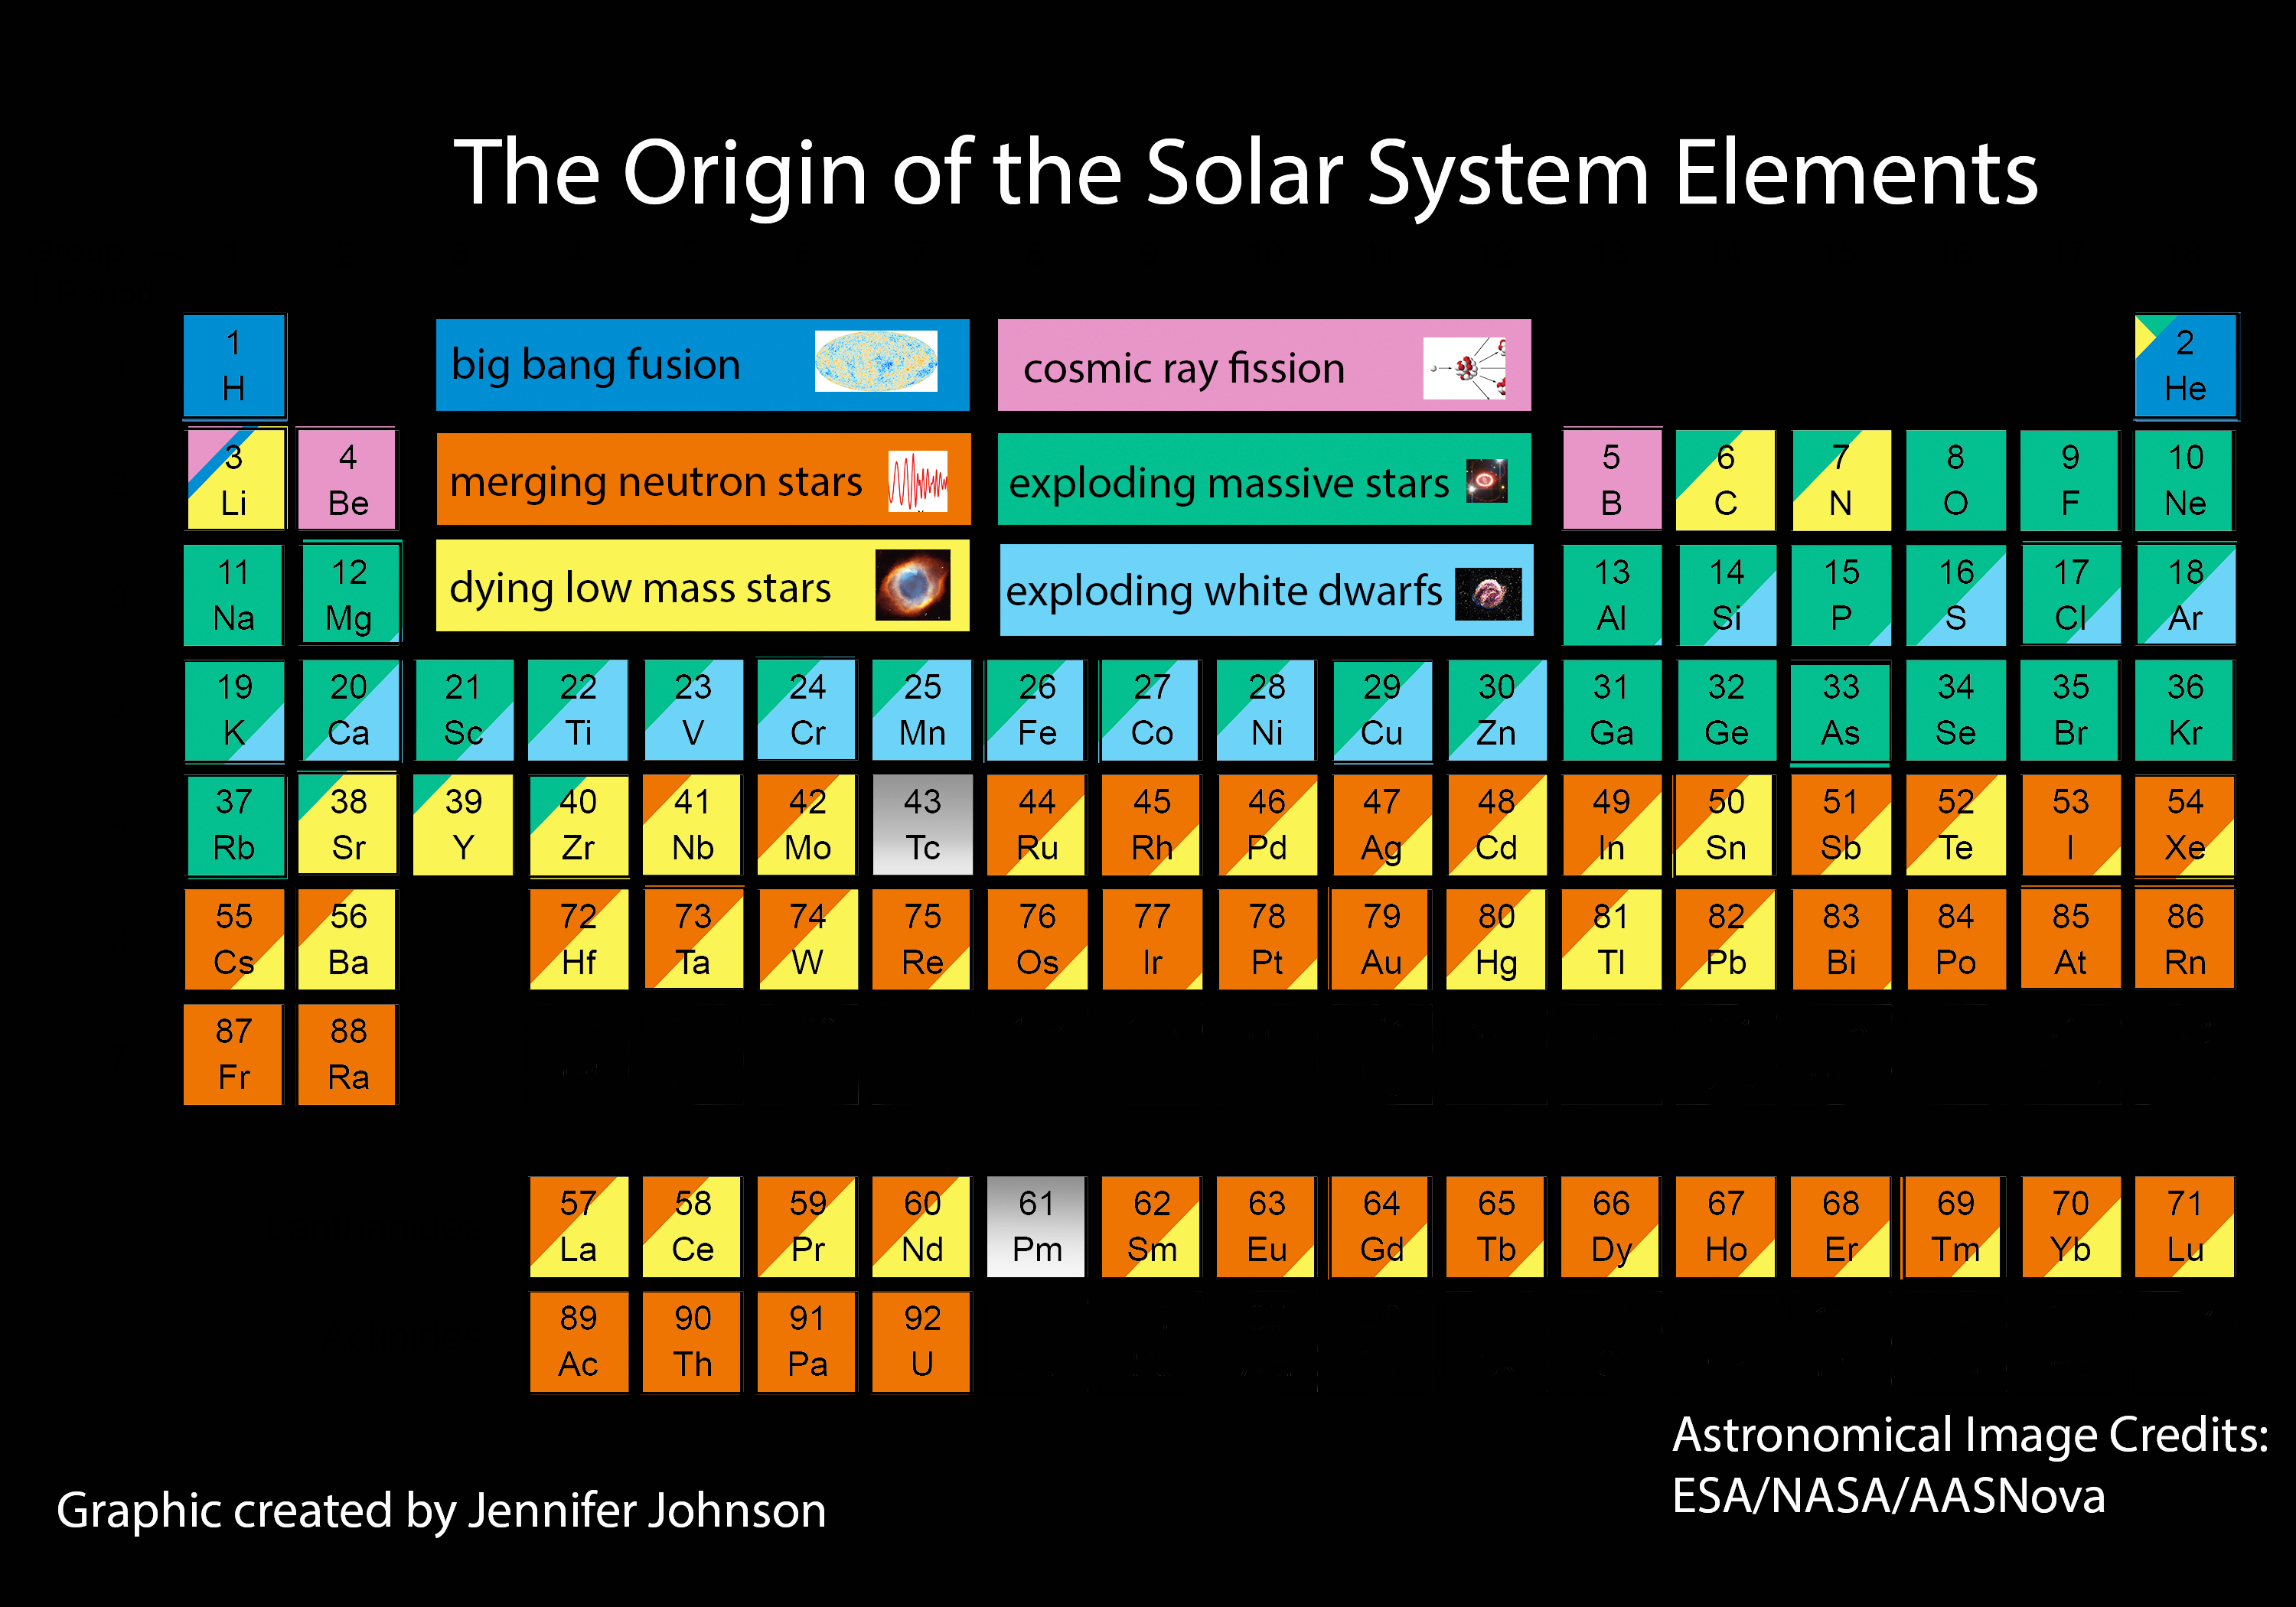
\includegraphics[width=0.7\linewidth]{8_periodic}
	\caption{Своеобразная таблица Менделеева}
	\label{fig:8_periodic}
\end{figure}

Разберем по цветам(пойду по строчкам):

\colorbox{Blue}{Big bang fusion} - слияние Большого взрыва; это те элементы, которые были до существования первых звёзд.

\colorbox{CarnationPink}{Cosmic ray fission} - это \href{https://en.wikipedia.org/wiki/Cosmic_ray_spallation}{"Реакция скалывания"}. Они происходят уже вне звёзд - сейчас существуют различные тяжелые элементы во вселенной. Космические лучи(частицы с высокой энергией), налетая на более тяжелые элементы, "модифицируют" их создавая как один из продуктов Бериллий/Бор/Литий. В звездах Бериллий и Бор не синтезируются - термоядерные реакции проскакивают с Гелия сразу до Углерода.

\colorbox{BurntOrange}{Merging neutron stars} - процесс слияния нейтронных звезд. Крайне важный и крайне редкий процесс(в нашей галактике - раз в ~30000 лет(по словам Попова)), который является источником самых тяжелых элементов.

\colorbox{SeaGreen}{Exploding massive stars} - \textbf{гравитационный коллапс} ядра массивной звезды, при котором часть оболочки сбрасывается, тем самым выбрасывая новые элементы. Происходят в нашей галактике раз в ~30 лет.

\colorbox{Yellow}{Dying low mass stars} - умирающие маломассивные звезды. Элементы синтезируются в оболочках этих красных гигантов. Взрыва не происходит - недостаточно массы, но звезда превращается в белый карлик, сбрасывая с себя оболочку которую мы называем планетарной туманностью.

\colorbox{Cyan}{Exploding white dwarfs} - термоядерный взрыв белого карлика. В основном синтезируются элементы группы Железа.

\subsection{Основные термоядерные реакции}

Теперь поговорим о термоядерных реакциях, происходящих в этих процессах. Нам \textbf{не важно} то, что происходит в ядрах звёзд! Потому что синтезирующиеся там элементы в этом ядре и остаются, например, создавая в конце жизни звезды углеродно-кислородный белый карлик(судьба нашего Солнца). Выделяют два основных процесса:

\begin{enumerate}
	\item S-процесс - Slow, медленный
	\item R-процесс - Rapid, быстрый
\end{enumerate}

S-процесс идёт в оболочках звезд-гигантов. Есть два процесса, создающих свободные нейтроны в звезде(рис. \ref{fig:8_neutrons}). Эти нейтроны легко проникают в ядра(у них нет заряда), увеличивая массу ядра, а затем, подвергаясь бета-распаду, синтезируют элементы с все большим зарядом. Так получаются элементы массой до ~100 и от ~138 до ~208. Процесс может идти миллионы лет.

\begin{figure}[H]
	\begin{subfigure}
		\centering
		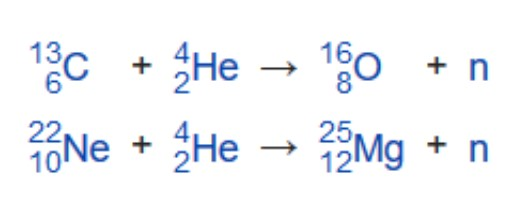
\includegraphics[width=0.7\linewidth]{8_neutrons}
		\caption{Реакции с выделением свободных электронов}
		\label{fig:8_neutrons}
	\end{subfigure}
	
	\begin{subfigure}
		\centering
		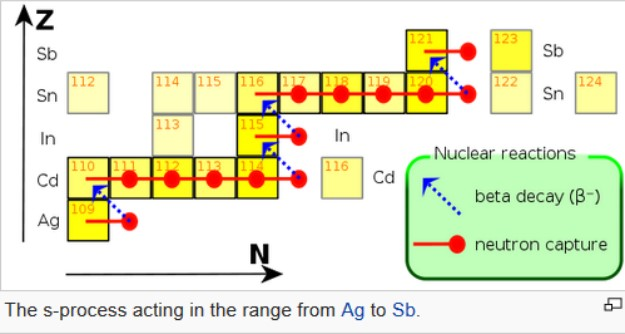
\includegraphics[width=0.7\linewidth]{8_slow}
		\caption{Пример S-процесса}
		\label{fig:8_slow}
	\end{subfigure}

	\label{fig:8_s_process}
\end{figure}

R-процесс идёт во вспышках сверхновых и при слиянии нейтронных звёзд. Временной масштаб тут намного меньше S-процесса: речь идет о секундах. Происходит всё при высокой плотности нейтронов, в результате получаются насыщенные нейтронами ядра, заряд ядра как и в случае медленного процесса увеличивается засчет бета распада. В результате получаются элементы вплоть до Урана.

\begin{figure}[H]
	\centering
	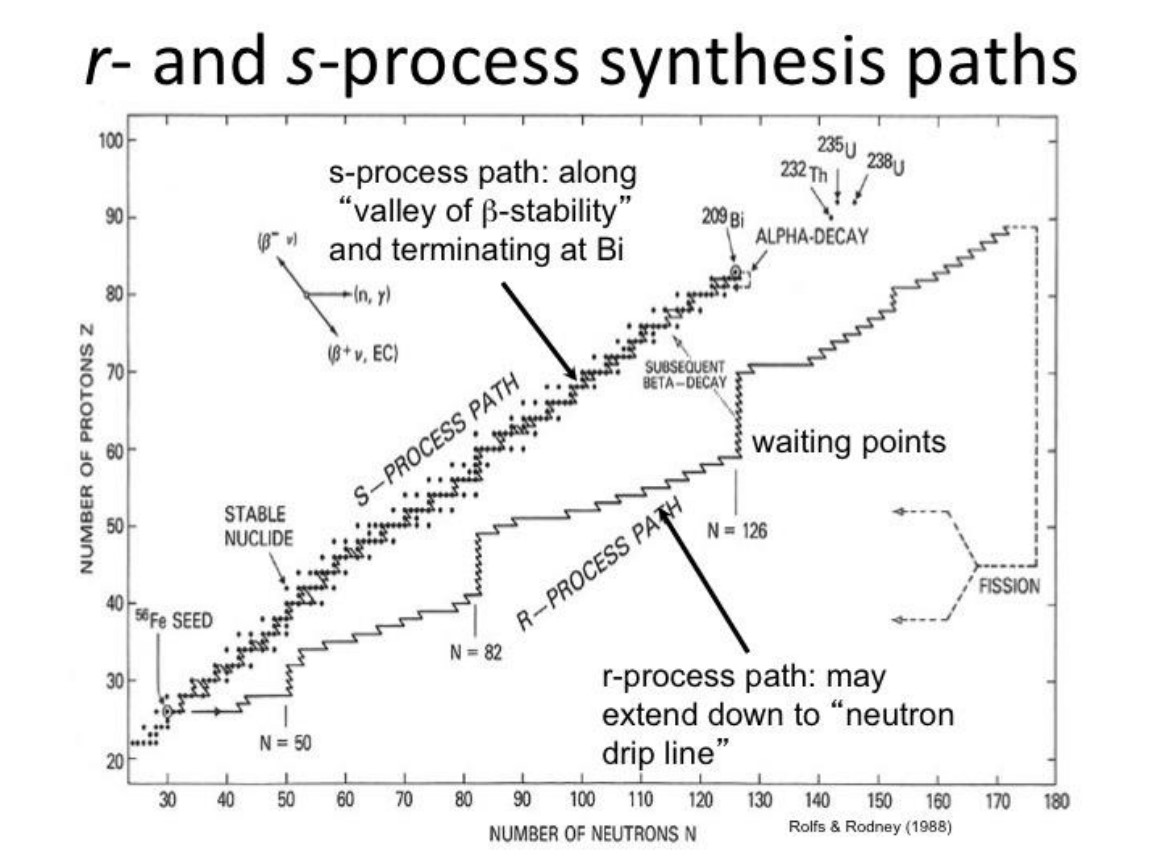
\includegraphics[width=0.7\linewidth]{8_comparison}
	\caption{Сравнение путей по которым могут идти s- и p- процессы}
	\label{fig:8_comparison}
\end{figure}
